\section{Exercise 6: Home Assistant}
The last exercise is about \textit{Home Assistant}. 
There are several tasks defined in the sheet about how to setup and use some features of \textit{Home Assistant}.

\subsection{Task 1: Setup}
As \textit{Home Assistant} recommends to use a Raspberry Pi to run the \textit{Home Assistant} server 
which is in my opinion more realistic than using a local virtual machine, i decided to use a Raspberry Pi 3B+ 
to run the \textit{Home Assistant} server. Image belows shows the \textit{Home Assistant} setup after the system was 
installed like described \href{https://www.home-assistant.io/installation/raspberrypi}{\textit{here}}.

\begin{figure}[H]
    \centering
    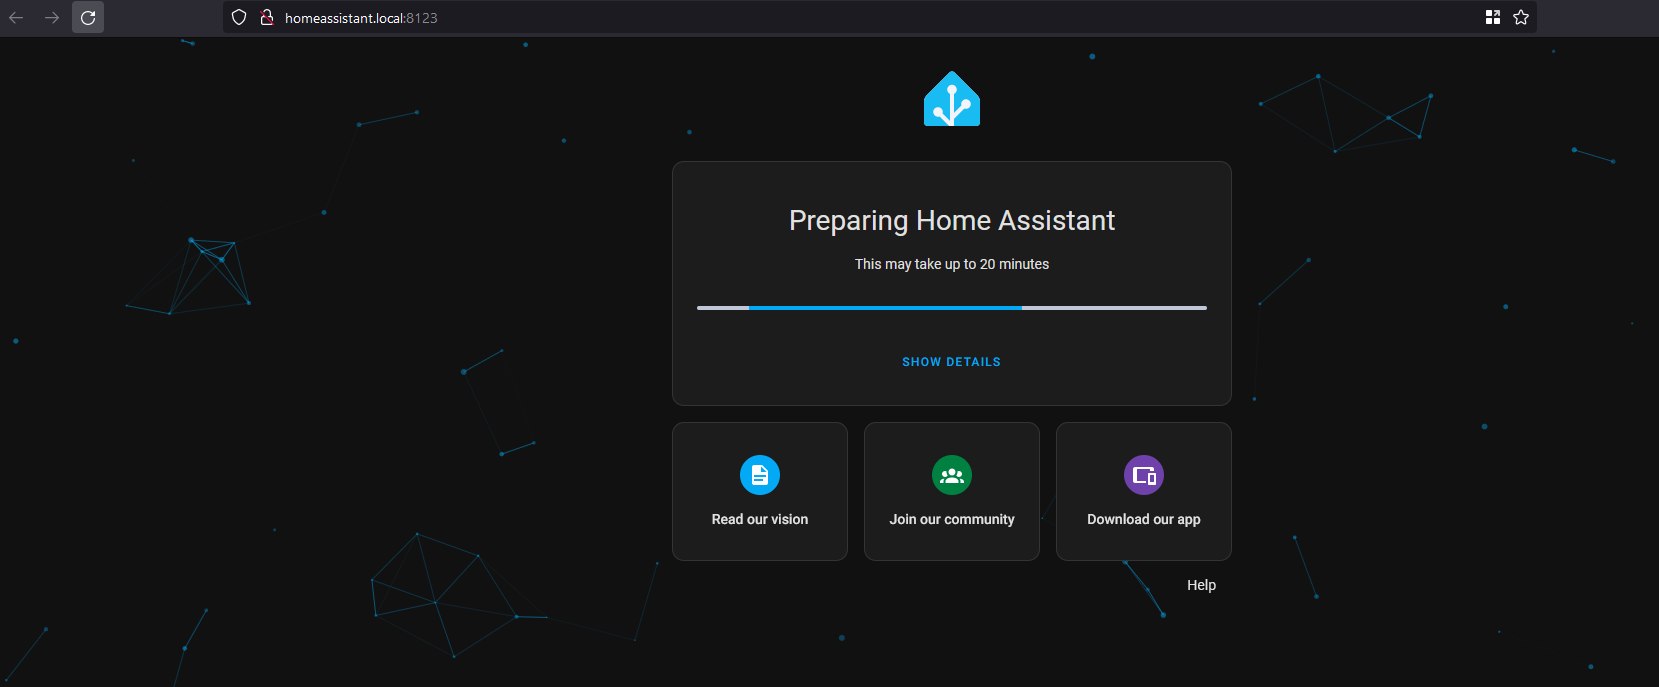
\includegraphics[width=1\textwidth]{exercise_home-assistant/setup.png}
    \caption{Home Assistant Setup}
    \label{fig:home_assistant_setup}
\end{figure}

After the setup was done the dashboard will be shown as seen in the image below.

\begin{figure}[H]
    \centering
    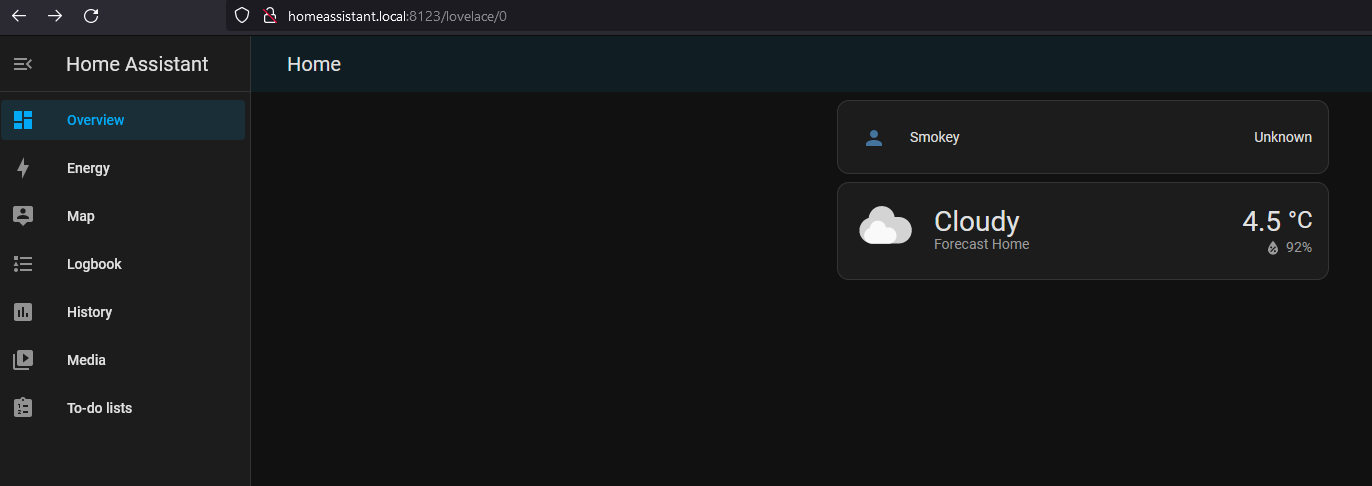
\includegraphics[width=1\textwidth]{exercise_home-assistant/dashboard_blank.png}
    \caption{Home Assistant Dashboard}
    \label{fig:home_assistant_dashboard}
\end{figure}

\subsection{Task 2: Add first service}
As first service it is required to add the \textit{AccuWeather} service to \textit{Home Assistant}.
This was mainly done like described in the tutorial \href{https://www.home-assistant.io/integrations/accuweather}{\textit{here}}.
Even if the default dashboard already contains a weather widget, i added this one to the dashboard as well.
Images below shows the successfully created \textit{AccuWeather Service} and the dashboard with the new widget.

\begin{figure}[H]
    \centering
    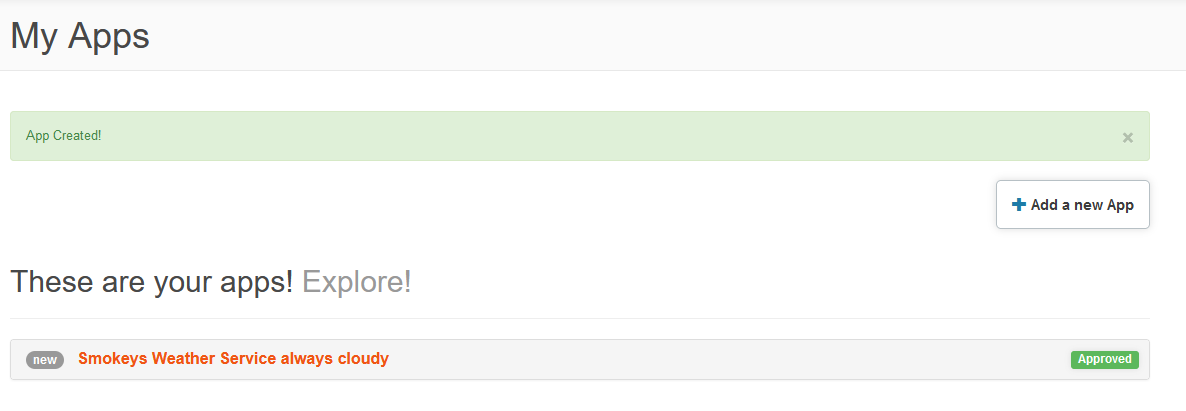
\includegraphics[width=1\textwidth]{exercise_home-assistant/accuweather.png}
    \caption{Home Assistant AccuWeather Service}
    \label{fig:home_assistant_accuweather_service}
\end{figure}

\begin{figure}[H]
    \centering
    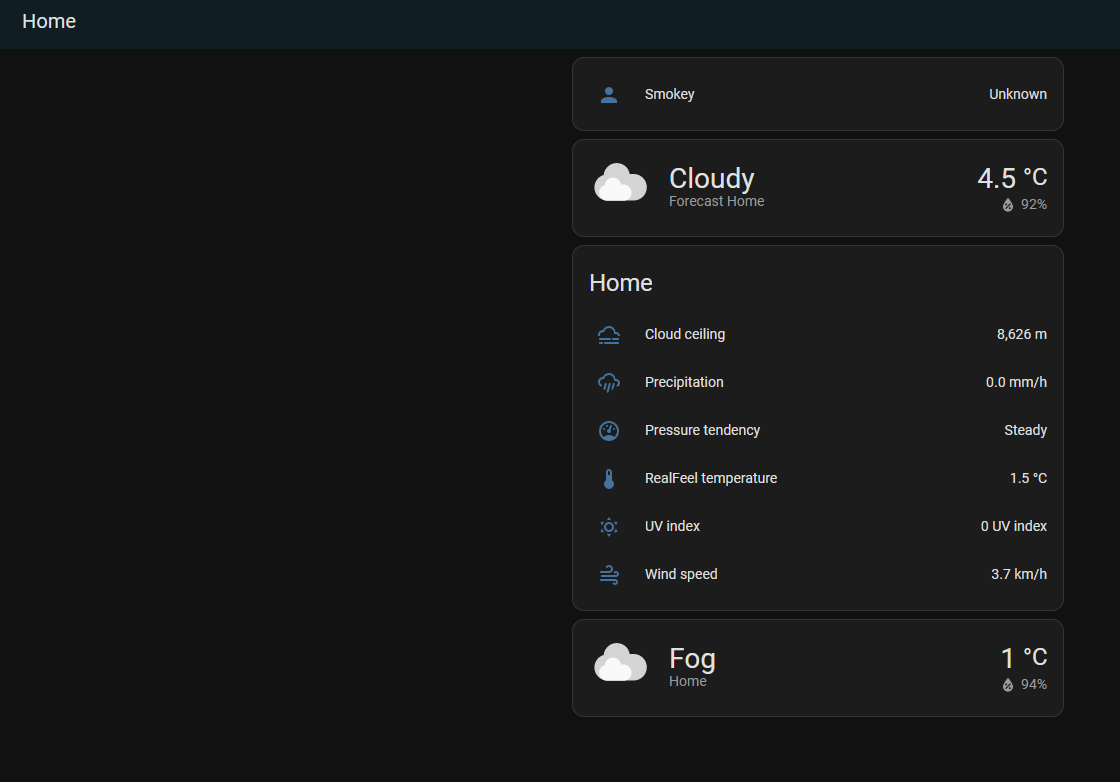
\includegraphics[width=1\textwidth]{exercise_home-assistant/dashboard_accuweather.png}
    \caption{Home Assistant Dashboard with AccuWeather Widget}
    \label{fig:home_assistant_dashboard_accuweather}
\end{figure}

\subsection{Task 3: Add first automation}
The third task is about adding the first automation to \textit{Home Assistant}.
Therefore it will be required to create a Telegram bot and add it to \textit{Home Assistant}. As i am not using 
Telegram i decided to use the \textit{Discord} bot instead. This was done like described in the tutorial 
\href{https://www.home-assistant.io/integrations/discord}{\textit{How to add discord bot}}.

After creating the new Discord application as described it will be shown in the Discord developer portal like 
shown in the image below.

\begin{figure}[H]
    \centering
    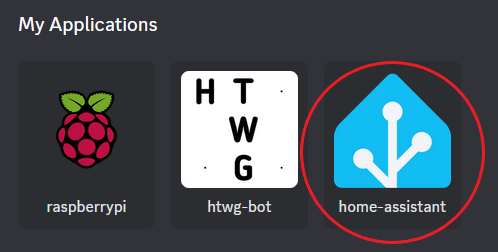
\includegraphics[width=1\textwidth]{exercise_home-assistant/discord_app.png}
    \caption{Discord Bot App View}
    \label{fig:discord_bot}
\end{figure}

After adding the Discord bot to \textit{Home Assistant} via the \textit{Devices \& services Integration} and to a 
private Discord server i used other bots before i was able to create a first automation.
Therefore the \textit{Developer Tools} were used to change the \textit{notification} service like shown in the 
image below.

\begin{figure}[H]
    \centering
    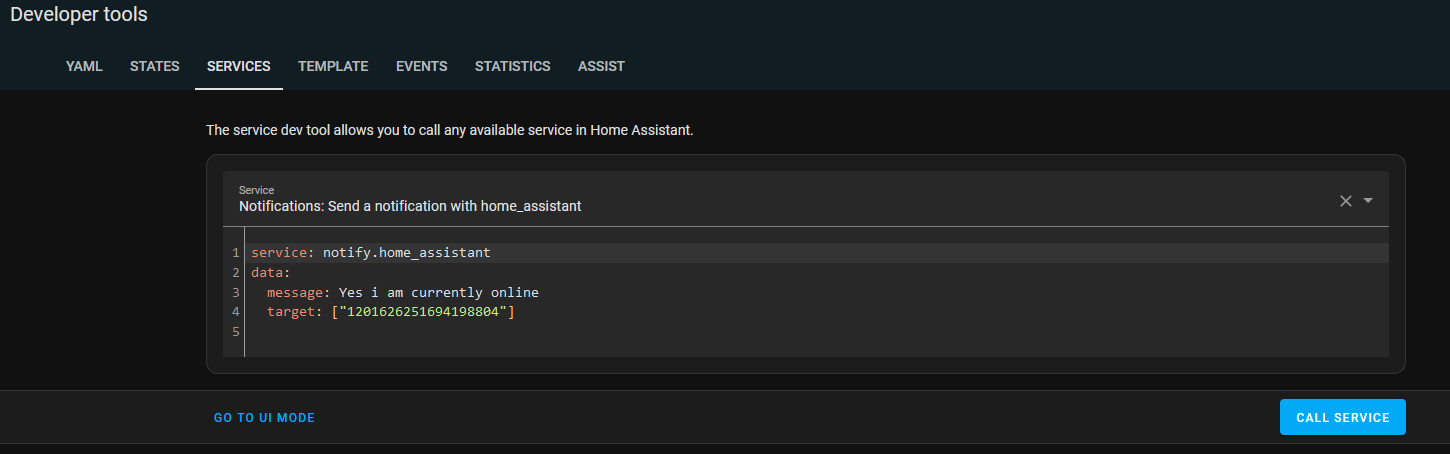
\includegraphics[width=1\textwidth]{exercise_home-assistant/service_yaml.png}
    \caption{Home Assistant Notification Service}
    \label{fig:home_assistant_notification_service}
\end{figure}

The target which is used in the \textit{target} field is the channel id of the channel where the Discord bot will 
send the messages to. Testing the service via the \textit{Call Service} button will send a message to the Discord 
channel like shown in the image below.

\begin{figure}[H]
    \centering
    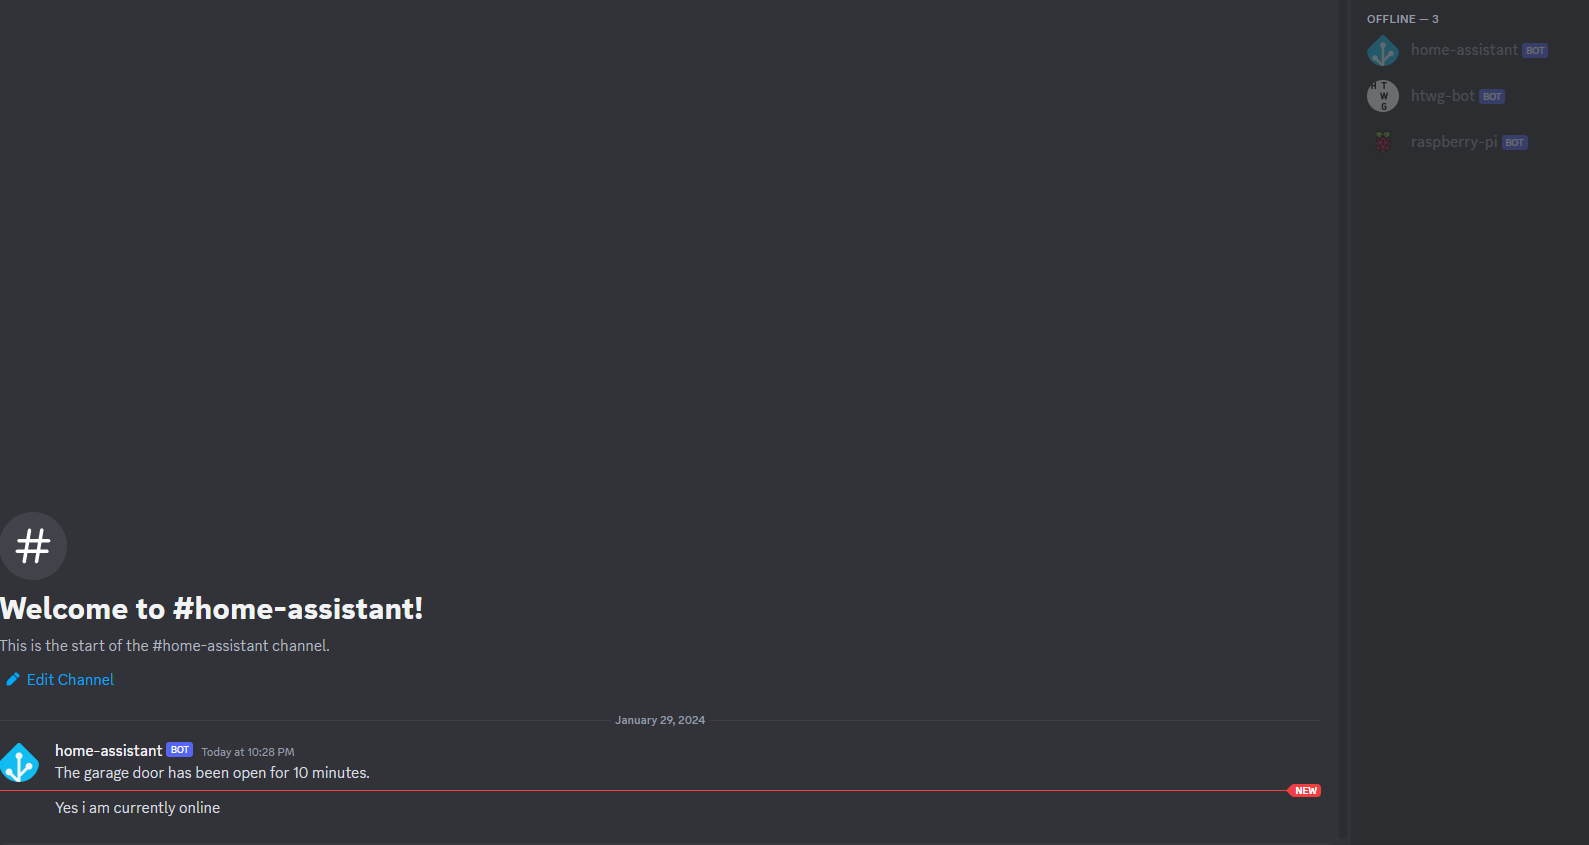
\includegraphics[width=1\textwidth]{exercise_home-assistant/bot_message.png}
    \caption{Discord Message from Home Assistant}
    \label{fig:discord_message}
\end{figure}


\subsection{Task 4: Add a periodical automation}
The fourth task is about adding a periodical automation to \textit{Home Assistant}.
Therefore the previous created notification service will be used to send a message to the Discord channel periodically.
Therefore I decided to use a message pattern like shown in the image bellow which will check the sun state and read the 
temperature data from the \textit{AccuWeather} service.
At the current version the notification will be send only once at minute 5 of every hour but can easily be extended to 
send the message every 5 minutes or every hour by adding more \textit{trigger} sections to the automation.

\begin{minted}
  [
    frame=lines,
    framesep=2mm,
    baselinestretch=1.2,
    linenos
  ]
  {C}

  trigger:
  - platform: time_pattern
    minutes: "5"
  - platform: time_pattern
    minutes: "10"
  ...
\end{minted}

The result of the automation can be seen in the image below as well as the discord notification which was send to the 
channel.

\begin{figure}[H]
    \centering
    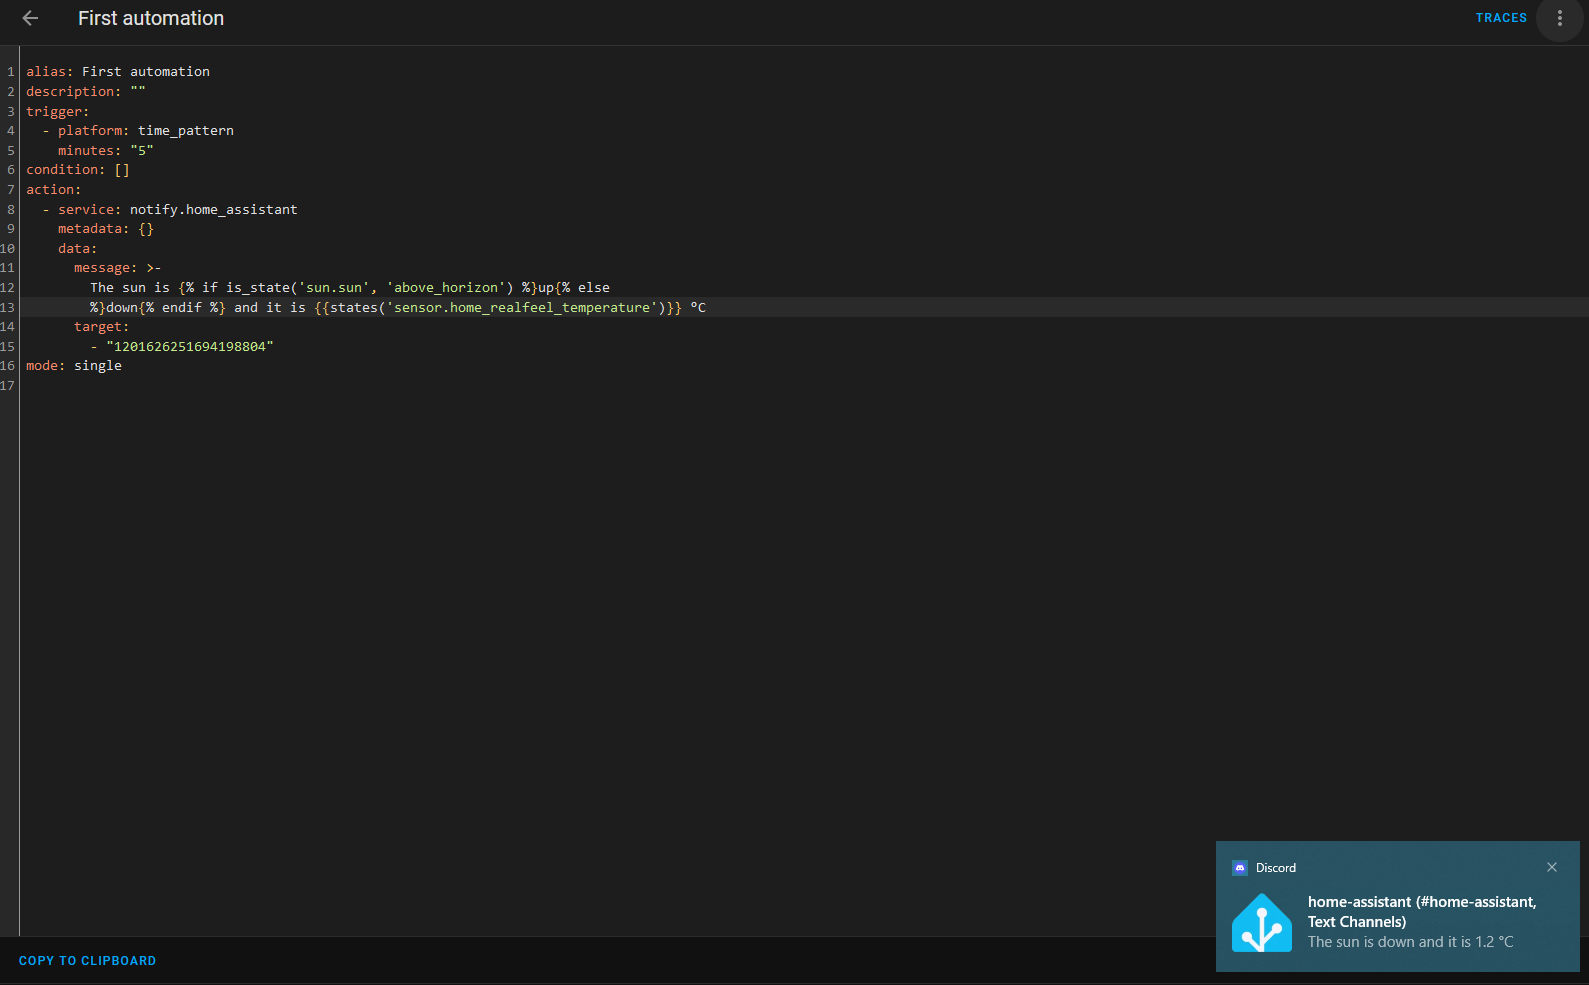
\includegraphics[width=1\textwidth]{exercise_home-assistant/automation.png}
    \caption{Discord Periodical Message from Home Assistant}
    \label{fig:discord_periodical_message}
\end{figure}